\section{The original pipeline, corrected}
\label{sec:baseline}

\subsection{Pipeline and fixes}

The original pipeline averaged the channels of each window, z-scored it, decomposed it with EMD-signal 1.9.0 \cite{laszuk2017}, and computed one of three features of the IMFs (variance, histogram entropy, or mean absolute instantaneous frequency). It classified with $k$-nearest neighbors (KNN, $k = 5$) under Pearson, Euclidean, and Itakura--Saito distances on one stratified 70/30 split of windows (seed 42), and clustered with $k$-means on the raw features, where the distance only scored the silhouette. A rerun of the March code on the March caches, which are not part of this repository, reproduced its values, so the errors were in the method and the report and not in the run.

The fixes are three. The EMD routine returns the IMFs followed by a residue row, and the original code counted the residue as an IMF and zero-padded every window to eight rows. The corrected pipeline keeps the residue apart and uses the first four true IMFs, with no padding (Fig.~\ref{fig:imf} shows one window). The last window of each EEGMAT recording was a padded tail, and three EEG MMI subjects were read at the wrong sampling rate. Both are removed (Section~\ref{sec:data}).

\begin{figure}[t]
\centering
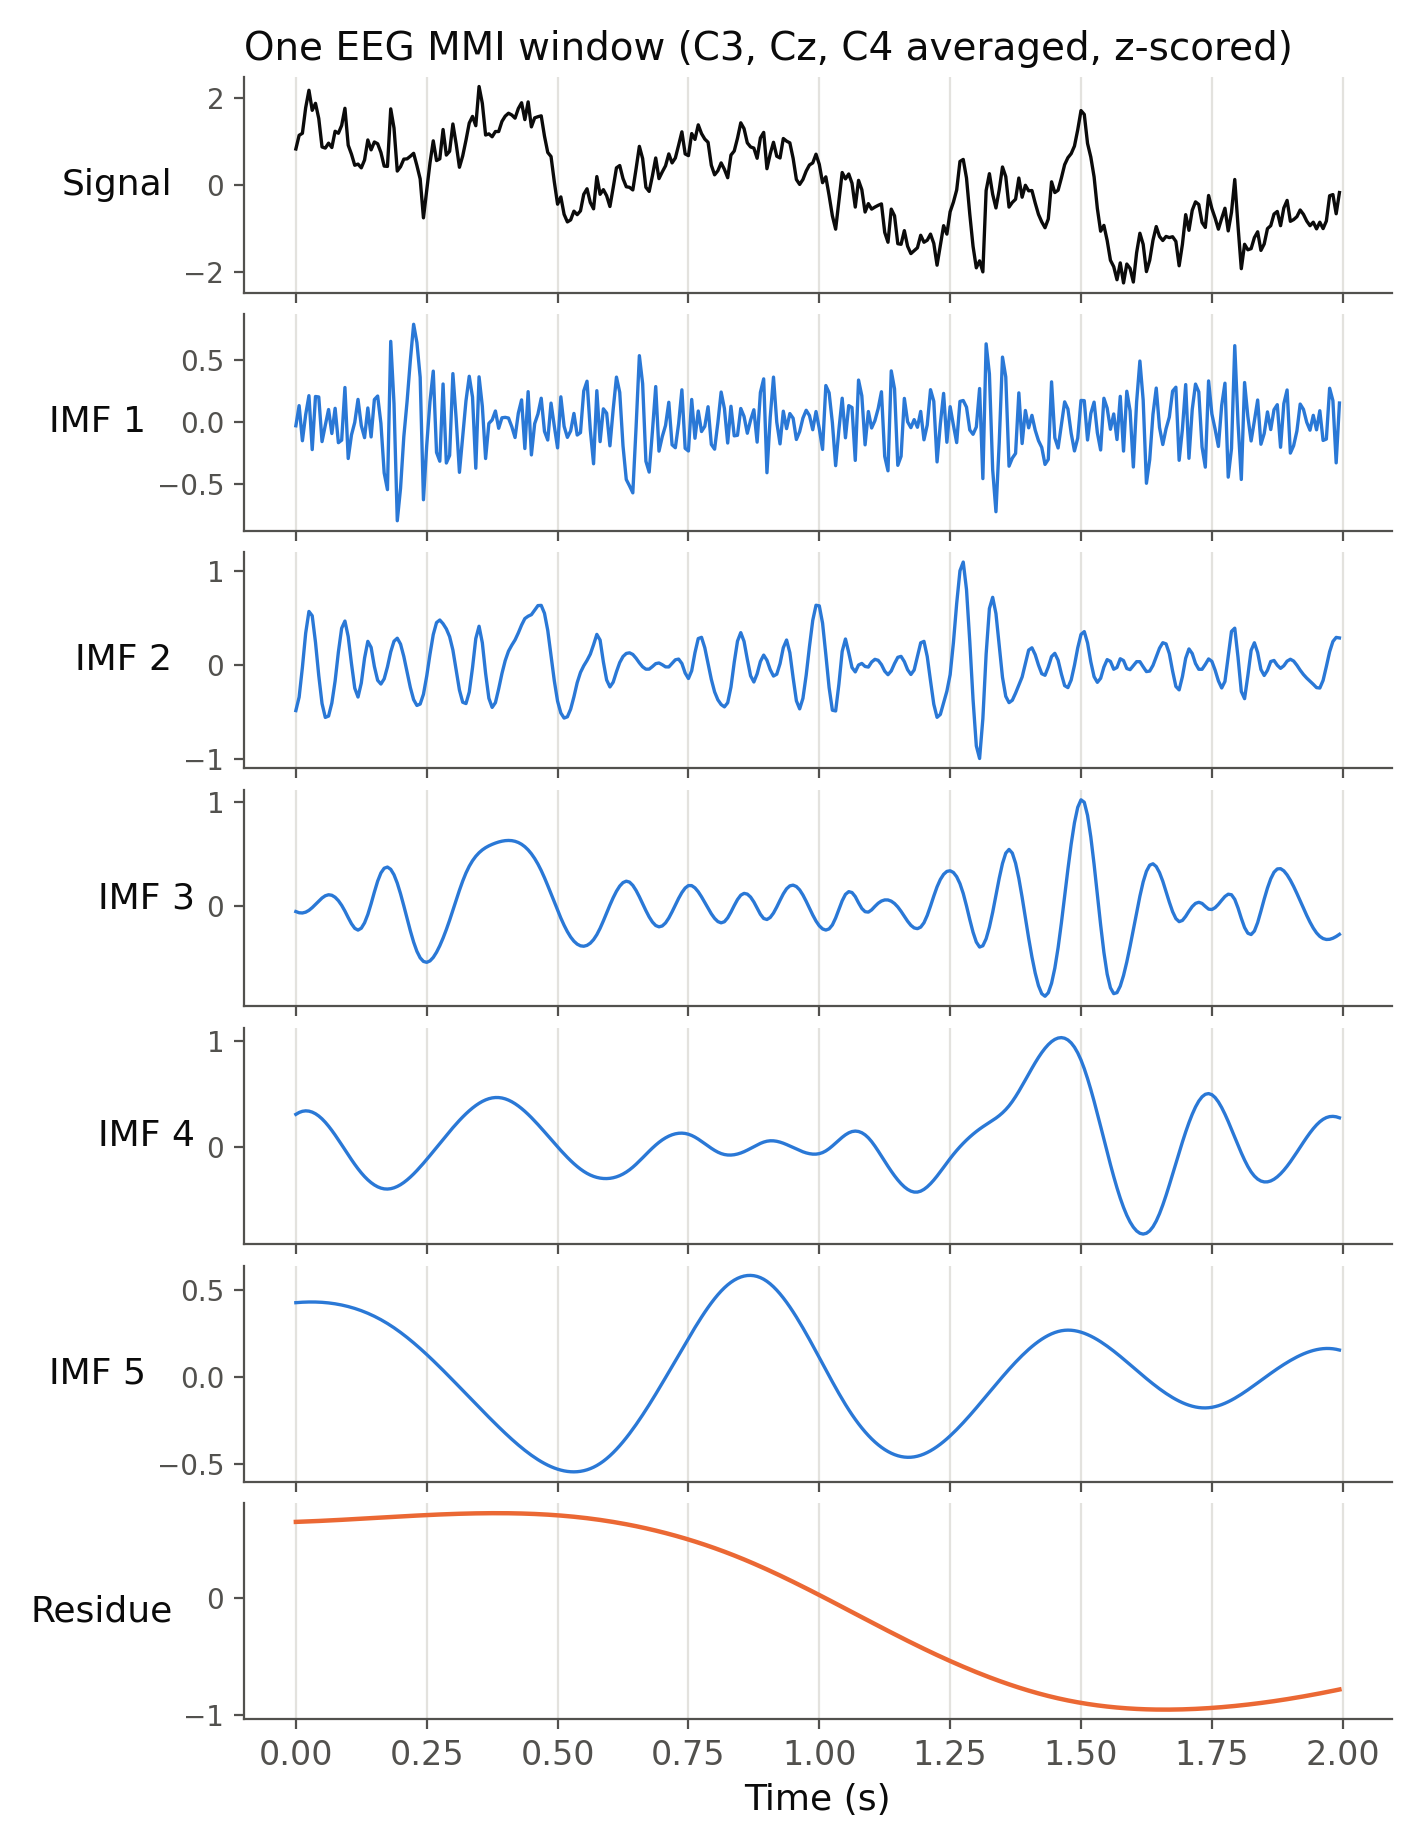
\includegraphics[width=0.85\columnwidth]{../results/study/figures/fig7_imf_example.png}
\caption{One EEG MMI window: the signal, its five IMFs, and the residue.}
\label{fig:imf}
\end{figure}

\subsection{Results}

Table~\ref{tab:baseline} gives the classification results. On motor imagery, the corrected baseline is at chance: balanced accuracy runs from \N{blr:eeg_mmi:bacc:min} to \N{blr:eeg_mmi:bacc:max} on EEG MMI (chance 0.50) and from \N{blr:bci_civ_2a:bacc:min} to \N{blr:bci_civ_2a:bacc:max} on BCI IV 2a (chance 0.25), the same as before the fixes. On EEGMAT, the best configuration (instantaneous frequency, Euclidean distance) has weighted F1 \N{bl:eeg_ma:inst_freq:euclidean:f1} and accuracy \N{bl:eeg_ma:inst_freq:euclidean:accuracy}, against \N{ar:corrected:f1} and \N{ar:corrected:acc} for always predicting rest, and balanced accuracy \N{bl:eeg_ma:inst_freq:euclidean:bacc}. The lowest corrected weighted F1 on EEGMAT is below the always-rest value. With one split and no uncertainty estimate, the differences among the original feature and distance pairs support no ranking.

\begin{table}[t]
\caption{The original pipeline: weighted F1 in the March run and after the fixes, and balanced accuracy after the fixes. Ranges over the nine feature and distance pairs. On EEGMAT, always predicting rest scores weighted F1 \N{ar:march:f1} on the March windows and \N{ar:corrected:f1} after the fixes.}
\label{tab:baseline}
\centering
\scriptsize
\setlength{\tabcolsep}{2.5pt}
\begin{tabular}{@{}lccc@{}}
\toprule
Data set & W. F1, March & W. F1, corrected & Bal. acc., corrected \\
\midrule
EEG MMI & 0.492--0.521 & 0.500--0.510 & 0.499--0.510 \\
BCI IV 2a & 0.222--0.262 & 0.220--0.273 & 0.225--0.278 \\
EEGMAT & 0.642--0.706 & 0.636--0.703 & 0.488--0.572 \\
\bottomrule
\end{tabular}

\end{table}

The clustering scores changed most. The entropy silhouettes of March (\N{mls:eeg_mmi:entropy:pearson} on EEG MMI with Pearson distance, against \N{bl:eeg_mmi:entropy:pearson:silhouette} after the fixes) were measuring the padding: $k$-means on the entropy features grouped windows by how many rows EMD returned, with an adjusted Rand index (ARI) against the row count of \N{cl:eeg_mmi:F0_ent:kmeans:pearson:ari_f0_row_count} (EEG MMI), \N{cl:bci_civ_2a:F0_ent:kmeans:pearson:ari_f0_row_count} (BCI IV 2a), and \N{cl:eeg_ma:F0_ent:kmeans:pearson:ari_f0_row_count} (EEGMAT) on the corrected windows. Against the classes, the ARI is between about \N{blc:all:ari_min} and \N{blc:all:ari_max} in every row. A silhouette is printed here only next to the ARI, because the corrected silhouettes are no better evidence: EEGMAT instantaneous frequency scores \N{bl:eeg_ma:inst_freq:euclidean:silhouette} with Euclidean distance and an ARI against the classes of \N{bl:eeg_ma:inst_freq:euclidean:ari}.

A permutation null for the window split (200 shuffles for each of three configurations, pooled: band power per channel with linear discriminant analysis (LDA) and with Euclidean KNN, and the original variance features with Euclidean KNN) puts the middle 95\% of balanced accuracy at \N{snp:eeg_mmi:lo} to \N{snp:eeg_mmi:hi} on EEG MMI, \N{snp:bci_civ_2a:lo} to \N{snp:bci_civ_2a:hi} on BCI IV 2a, and \N{snp:eeg_ma:lo} to \N{snp:eeg_ma:hi} on EEGMAT; Fig.~\ref{fig:null} shows the null of weighted F1 with the March and corrected values. The null shuffles window labels freely, which assumes that windows are exchangeable; windows that share subjects or recordings are not, so clearing it does not show task information.

\begin{figure}[t]
\centering
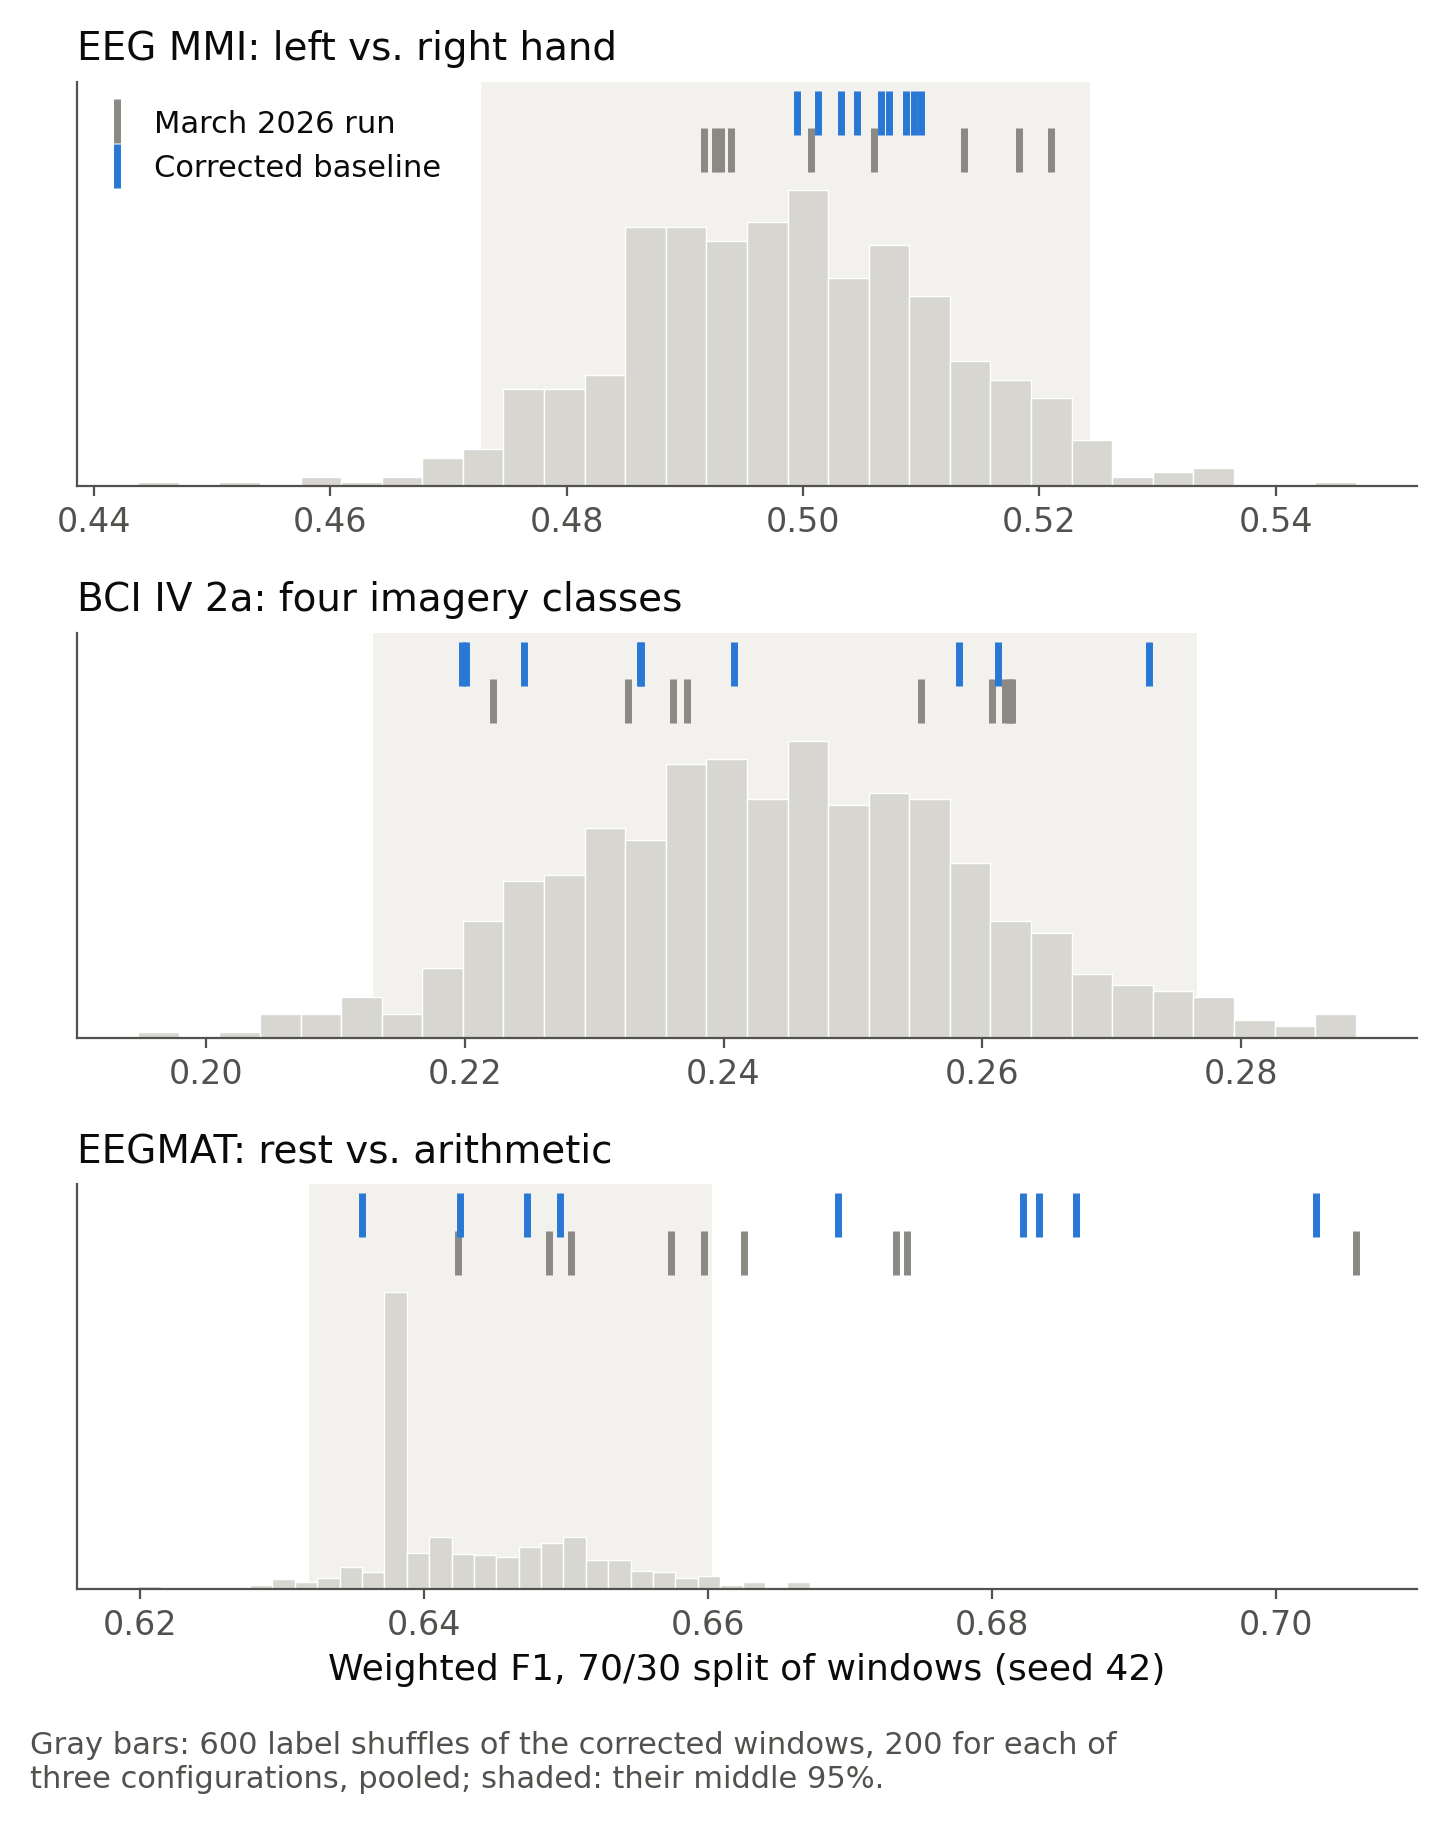
\includegraphics[width=0.85\columnwidth]{../results/study/figures/fig6_null.png}
\caption{Null distribution of weighted F1 for the window split (600 shuffles, 200 for each of three configurations, pooled), with the March values and the corrected values marked. The null is built on the corrected windows. The narrow EEGMAT peak is the null of the LDA configuration. Always predicting rest scores \N{ar:corrected:f1} on the corrected EEGMAT windows and \N{ar:march:f1} on the March ones, so the March values sit against a null for slightly different windows.}
\label{fig:null}
\end{figure}
